\documentclass[addpoints]{exam}
\usepackage{amsmath, amsfonts}
\usepackage{enumitem}
\usepackage{geometry}
\usepackage{hyperref}
\usepackage{tikz}

\usetikzlibrary{shapes,snakes}
\usetikzlibrary{automata,positioning,arrows}

% Header and footer.
\pagestyle{headandfoot}
\runningheadrule
\runningfootrule
\runningheader{CS 212}{HW 1}{Fall 2021}
\runningfooter{}{Page \thepage\ of \numpages}{}
\firstpageheader{}{}{}

\boxedpoints
\noprintanswers

\tikzset{
  >=stealth,
  node distance=3cm, 
  every state/.style={thick, fill=gray!10}, 
  initial text=$ $ 
}

\title{Homework 1}
\author{CS 212 Nature of Computation\\Habib University\\Fall 2021}
\date{Due: 2359h on Friday, 1 October}

\begin{document}
\maketitle

\begin{questions}
\question For each of the languages specified below, draw the state diagram of a DFA that recognizes it. In all cases $\Sigma = \{0,1\}$.
  \begin{parts}
  \part[05] $L = \{ w : w \text{ begins with $1$ and ends with $0$}\}$
  \part[05] $L = \{ w: w \text{ does not contain $100$ as substring} \}$
  \part[05] $L = \{ w : w \text{ starts with $0$ and has odd length} \}$
  \end{parts}
  
\question Convert the following NFA's to equivalent DFA's. Make sure to remove unnecessary states from the DFA.
  \begin{parts}
  \part[10] $\null$\\
    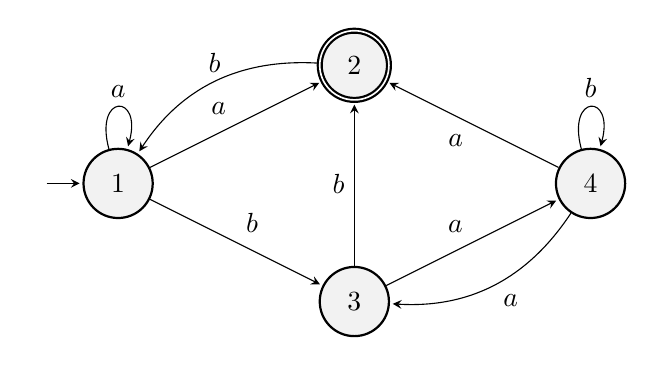
\begin{tikzpicture}[shorten >=1pt,node distance=2cm,on grid,auto] 
      \node[state,initial] (q_1) at (0, 0)  {$1$}; 
      \node[state, accepting] (q_2) at (3, 1.5) {$2$}; 
      \node[state] (q_3) at (3, -1.5)  {$3$};
      \node[state] (q_4) at (6, 0) {$4$};
      
      
      \path[->] (q_1) edge [loop above] node {$a$} (q_1)
      (q_1) edge node {$a$} (q_2)
      (q_2) edge [bend right] node[above] {$b$} (q_1)
      (q_1) edge node {$b$} (q_3)
      (q_3) edge node {$b$} (q_2)
      (q_3) edge node {$a$} (q_4)
      (q_4) edge node {$a$} (q_2)
      (q_4) edge [bend left] node {$a$} (q_3)
      (q_4) edge [loop above] node {$b$} (q_4);
    \end{tikzpicture}

  \part[10] $\null$\\
    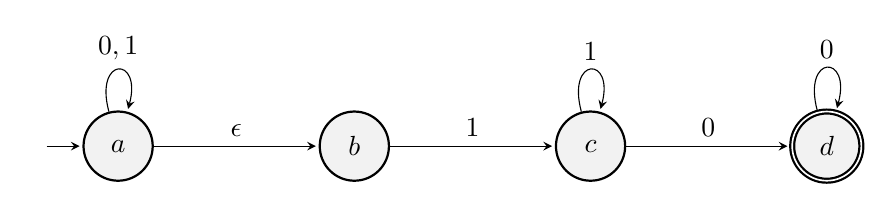
\begin{tikzpicture}[shorten >=1pt,node distance=2cm,on grid,auto] 
      \node[state,initial] (q_1) at (0, 0)  {$a$}; 
      \node[state] (q_2) at (3, 0) {$b$}; 
      \node[state] (q_3) at (6, 0)  {$c$};
      \node[state,accepting] (q_4) at (9, 0) {$d$};
      
      
      \path[->] (q_1) edge [loop above] node {$0,1$} (q_1)
      (q_1) edge node {$\epsilon$} (q_2)
      (q_2) edge node {$1$} (q_3)
      (q_3) edge node {$0$} (q_4)
      (q_3) edge[loop above] node {$1$} (q_3)
      (q_4) edge[loop above] node {$0$} (q_4);
    \end{tikzpicture}
  \end{parts} 

  
\question For each of the languages specified below, draw the state diagram of a NFA that recognizes it. In all cases $\Sigma = \{0,1\}$.
  \begin{parts}
  \part[05] $L = \{ w : w \text{ contains the substring $1100$ or does not contain the substring $1010$} \}$
  \part[05] $ L= \{ 0^*1^*0^+\}$ i.e.,  that is the set of strings consisting of some number of $0$'s followed by some number of $1$'s followed by at least one $0$
  \end{parts}

\question Convert the following regular expressions to NFA's:
  \begin{parts}
  \part[05] $(0 \cup 1)^*000(0\cup 1)^*$
  \part[05] $(((00)^*(11))\cup 01)^*$
  \part[05] $\emptyset^*$		
  \end{parts}


\question[10] Let
  \[
    \Sigma_2 = \left\{ \begin{bmatrix} 0\\0 \end{bmatrix}, \begin{bmatrix} 0\\1 \end{bmatrix}, \begin{bmatrix} 1\\0 \end{bmatrix}, \begin{bmatrix} 1\\1 \end{bmatrix} \right\}.
  \]
  That is, $\Sigma_2$ contains all columns of 0s and 1s of height two. A string of symbols in $\Sigma_2$ gives two rows of 0s and 1s. Consider each row to be a binary number and let
  \[
    C = \{ w\in\Sigma_2^* \mid \text{ the bottom row of }w \text{ is 3 times the top row} \}.
  \]
  For example, $\begin{bmatrix} 0\\0 \end{bmatrix} \begin{bmatrix} 0\\1 \end{bmatrix} \begin{bmatrix} 1\\1 \end{bmatrix} \begin{bmatrix} 0\\0 \end{bmatrix} \in C$, but  $\begin{bmatrix} 0\\1 \end{bmatrix} \begin{bmatrix} 0\\1 \end{bmatrix} \begin{bmatrix} 1\\0 \end{bmatrix} \not\in C$. Show that $C$ is regular.

  
  \begin{EnvFullwidth}
    {\large\bf Bonus}\\
    The following question does not carry marks but is interesting to think about. Attempt it if you are interested.
  \end{EnvFullwidth}

\question[0] Let $A$ be a regular language. Define $\text{\textsc{skip-a-symbol}}(A)$ to be a language consisting of all strings that can be obtained by removing one symbol from a string in $A$. Thus 
  \[
    \text{\textsc{skip-a-symbol}}(A) =  \{ xz : xyz \in  A \text{ where } xz \in \Sigma^*, y \in \Sigma\}
  \]
  Show that the class of regular languages is closed under $\text{\textsc{skip-a-symbol}}$ operation. Give a formal proof by construction. 
  
\end{questions}

\end{document}

%%% Local Variables:
%%% mode: latex
%%% TeX-master: t
%%% End:
